% simple.tex - A simple article to illustrate my intermediary report.

%preamble

 
\documentclass{article}
\usepackage{graphicx}
\graphicspath{ {C:\Users\Dani\Desktop\Raport} }
\usepackage{color}
\usepackage[utf8]{inputenc}
\usepackage{hyperref}
\usepackage{}
\usepackage{algorithmic}
\usepackage{algorithm}
\usepackage{txfonts}
\usepackage[romanian]{babel}
\hypersetup{
    colorlinks=true,
    linkcolor=blue,
    filecolor=magenta,      
    urlcolor=cyan,
}
\usepackage[T1]{fontenc}
\usepackage{amsmath}

\usepackage[noend]{algpseudocode}

\begin{document}

%top matter

\title{Tema de cas\u{a}\\-Drum in grid- \\}
\author{\Large{Trandafir Daniela-Georgiana }}
\date{May 2020}


\maketitle

\begin{tabbing}
\\
\\
\\
\\
\indent{Profesor:}  \=\href{http://software.ucv.ro/~cbadica}{Costin B\u{a}dic\u{a}} \\
\indent{Profesor laborator: Cristinel Ungureanu} 
\\
\\
\\
\\
\end{tabbing}

% abstract

\begin{itemize}
  \item Specializarea : Calculatoare cu predare \^{i}n limba Rom\^{a}n\u{a}
  \item Anul : $I$
  \item Grupa : 1.3 B
\end{itemize}
\\
\\\
\\\
\\\
\\\
\\\
\\ \  
\\
\thanks{UCV Facultatea de Automatic\u{a},Calculatoare \c{s}i Electronic\u{a}}
\vfill


\pagebreak

%sections

\section{Enun\c{t}ul Problemei}
\textbf{Drum in grid}
\\Se consider\u{a} un teren \^{i}n form\u{a} de grid p\u{a}tratic de dimensiuni $N\times N$. Fiecare loca\c{t}ie din grid este caracterizat\u{a} printr-un num\u{a}r \^{i}ntreg pozitiv ce reprezint\u{a} cota loca\c{t}iei respective ( \^{i}n\u{a}l\c{t}imea unui punct de pe
teren fa\c{t}\u{a} de un plan orizontal de referint\c{t}\u{a}). Se cere g\u{a}sirea unui drum
din col\c{t}ul din st\^{a}nga-sus al terenului p\^{a}n\u{a} \^{i}n col\c{t}ul din dreapta-jos al
terenului astfel \^{i}nc\^{a}t:
\par i) deplasarea de-alungul drumului se face doar c\u{a}tre
dreapta sau \^{i}n jos; 
\par ii) costul drumului, calculat ca suma valorilor absolute
ale diferen\c{t}elor dintre cotele  consecutive de-alungul drumului, s\u{a}
fie minim\u{a}. Se vor implementa doi algoritmi diferi\c{t}i.
\section{Algoritmi}

 
 
\subsection{Algoritm I}
\begin{center}
\begin{tabbing}
min\_cost($n $) \\
1.\indent   $inf \leftarrow 2000000000$ \\
2.\indent {\bf For} \=$i=0,n$ {\bf do} \\
3.   \indent \>$sum\big[i]\big[0] \leftarrow inf$\\
4.    \indent \>$sum\big[0]\big[i] \leftarrow inf$\\
5. 6.       
\indent $sum\big[0]\big[1] \leftarrow  0$, $sum\big[1]\big[0]  \leftarrow 0$ \\
7.{\bf For} \=$i=1,n$ {\bf do} \\ 
		8.\>	{\bf For} \=$j=1,n$ {\bf do} \\ 
	9.		 \indent \>\>
			 
	 $sum\big[i]\big[j] \leftarrow minim\big(absolut\big(cost\big[i]\big[j],cost\big[i]\big[j-1]\big)+sum\big[i]\big[j-1], \\ absolut\big(cost\big[i]\big[j], cost\big[i-1]\big[j]\big) + sum\big[i-1]\big[j]\big)$ \\

 10. \indent  $result\leftarrow sum\big[n]\big[n] - cost\big[1]\big[1] $ \\
11.\indent {\bf Return:} result
\end{tabbing}
\end{center}
\\Complexitatea algoritmului este: $O(n^2)$ % regular O
\\\^{I}n urma gener\u{a}rii testului pentru timpul de execu\c{t}ie am obtinut urm\u{a}toarele rezultate:
\begin{figure}[h]
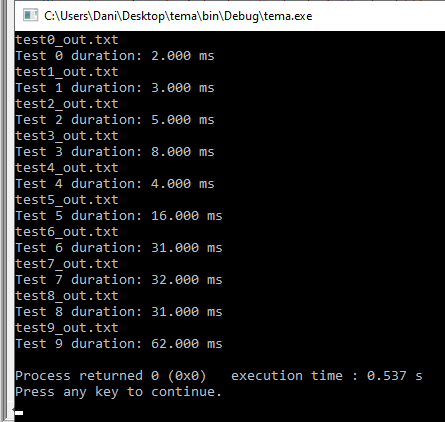
\includegraphics[width=5.25cm,height=5.25cm]{Figura1}
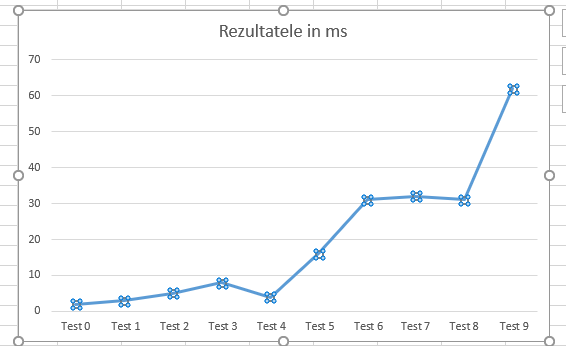
\includegraphics[width=7cm,height=5cm]{Grafic1}
\end{figure}


 
\subsection{Algoritm II}
\begin{center}
\begin{tabbing}
solve($n$) \\ 
\indent  $inf \leftarrow 2000000000$ \\
\indent $head.next \leftarrow NULL$ \\
\indent {\bf For} \=$i=0,n-1$ \\
			\indent \> {\bf For} \=$i=0,n-1$ \\
			 \indent \> \>
			  $d\big[i]\big[j] \leftarrow inf$ \\
		
\indent $d\big[0]\big[0] \leftarrow inf$ \\
\indent $aux.first \leftarrow 0, aux.second \leftarrow 0$ \\
\indent \textbf{push\_element\_end}\big(head,aux)\\

{\bf While} \=$ \textbf{list\_empty\big(head)} = 1 $ {\bf do} \\  
\indent \> $aux \leftarrow \textbf{pop\_element\_begining}\big(head)$ \\
\indent \>$i \leftarrow aux.first$ \\
\indent \> $j \leftarrow aux.second$ \\
    
  \indent  \>  {\bf If} $i+1 <n$ \\
        
        \indent \> \> \quad {\bf If} $d\big[i+1]\big[j]= inf$\\
        
            \indent \>\>\quad\quad $aux.first \leftarrow i+1$ \\
            \indent \>\>\quad\quad \ $aux.second \leftarrow j$ \\
             \indent \>\>\quad\quad \textbf{\textit push\_element\_end}\big(head,aux\big) \\
                
        \indent \> d\big[i+1]\big[j] = minim(d\big[i+1]\big[j], d\big[i]\big[j]+absolut\big(a\big[i]\big[j], a\big[i+1]\big[j]\big)\big) \\
  \\
\indent \>\> \If{j+1 <n} \\
    \indent \>\>\quad\If{d\big[i]\big[j+1] = inf} \\
   \indent \>\>\quad\quad$aux.first \leftarrow i$\\
     \indent \>\>\quad\quad $aux.second \leftarrow j+1$ \\
     \indent \>\>\quad\quad \textbf{\textit push\_element\_end}\big(head,aux\big) \\
\indent \> d\big[i]\big[j+1] = minim(d\big[i]\big[j+1], d\big[i]\big[j]+absolut\big(a\big[i]\big[j], a\big[i]\big[j+1]\big)\big) \\
\indent {\bf Return:} d[n-1][n-1]
\end{tabbing}
\end{center}
\\Complexitatea algoritmului este: $O(n^2)$ 
\\\^{I}n urma gener\u{a}rii testului pentru timpul de execu\c{t}ie am obtinut urm\u{a}toarele rezultate:
\begin{figure}[h]
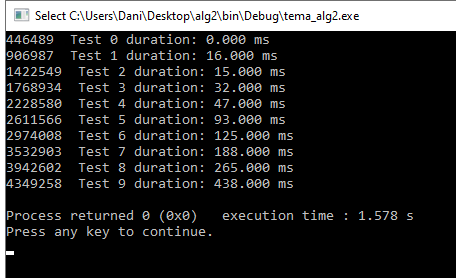
\includegraphics[width=7cm,height=5cm]{Figura2}
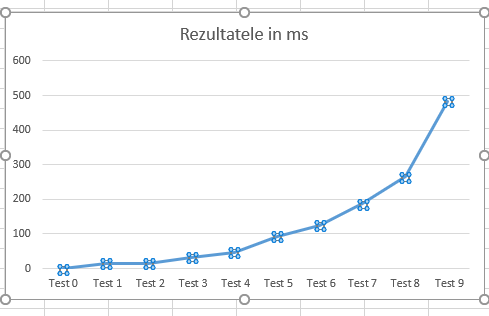
\includegraphics[width=7cm,height=5cm]{Grafic2}
\end{figure}

\section{Date experimentale}

\begin{center}
\begin{tabbing}
generator(n) \\
\indent \ \ \ \ \    $n \leftarrow \big(test+1)$ $*50$\\
\indent{\bf for} \=$linie = 1,n $ {\bf do}\\
\indent \> {\bf for} \=$coloana = 1,n $ {\bf do} \\
\indent \>\> rand()
\end{tabbing}
\end{center}
\\ Pentru generarea automat\u{a} am creat un modul \textbf{generator.c} pe care l-am introdus ca func\c{t}ie \^{i}n ambele programe.
\\Algoritmul genereaz\u{a}  dimensiunea matricei \textbf{n x n}, un num\u{a}r direct propor\c{t}ional cu num\u{a}rul testului
%% spun cum se formeaza n ul
, \c{s}i apoi valorile fiec\u{a}rui element, numere aleatorii \^{i}ntre 0 si RAND\_MAX.
\\Dat fiind intervalul de generare al func\c{t}iiei {\bf rand()} $\big(0,2^{15}-1\big)$ rezult\u{a} faptul c\u{a}
datele de intrare sunt valide pentru problema dat\u{a}.
\section{Proiectarea aplica\c{t}iei experimentale}
\subsection{Structura}
\\Aplica\c{t}ia creat\u{a} este organizat\u{a} \^{i}n module, fiecare con\c{t}in\^{a}nd func\c{t}ii particulare.
%de ce sunt semnificative pentru testele generate

\subsection{Date de intrare}
\\Datele de intrare sunt sub forma unei matrice p\u{a}tratice.Fiecare element din matrice reprezint\u{a} o loca\c{t}ie in grid si este caracterizat printr-un numar \^{i}ntreg pozitiv ce reprezint\u{a} cota loca\c{t}iei respective.
\subsection{Date de ie\c{s}ire}
\\Programul genereaz\u{a} o valoare minim\u{a} ce reprezint\u{a} costul drumului, calculat ca suma valorilor absolute ale diferen\c{t}elor dintre cotele loca\c{t}ilor consecutive de-alungul drumului.
\subsection{Modulele aplicatiei}
\\ $\Rightarrow$ \^{I}n cadrul func\c{t}ei main se citesc datele de intrare: valoarea <n> ce reprezint\u{a} dimensiunea matricei si apoi toate valorile din matrice. Se apeleaz\u{a} apoi func\c{t}ia pentru generarea rezultatului \c{s}i se afiseaz\u{a} rezultatul.
\\ $\Rightarrow$
\^{I}n cadrul func\c{t}iei homework1.c, respectiv homework2.c pentru al doilea algoritm se apleaz\u{a} toate func\c{t}iile necesare:

\par \textbf{I} 
\\ minim - func\c{t}ie care returneaz\u{a} minimul dintre dou\u{a} numere naturale;
\\absolut - functie care returneaz\u{a} diferen\c{t}a absolut\u{a} dintre dou\u{a} numere;
\\ solve - func\c{t}ia care creeaz\u{a} o matrice ce va fi populat\u{a} cu costurile minime pentru a ajunge la fiecare pozi\c{t}ie. Aceasta returneaz\u{a} valoarea final\u{a} prin parametrul <solve>.
\par \textbf{II}
\\ minim - func\c{t}ie care returneaz\u{a} minimul dintre dou\u{a} numere naturale;
\\absolut - functie care returneaz\u{a} diferen\c{t}a absolut\u{a} dintre dou\u{a} numere;
\\push\_element\_begining - func\c{t}ie care adaug\u{a} elemente la \^{i}nceputul unei cozi;
\\push\_element\_end - func\c{t}ie care adaug\u{a} elemente la finalul unei cozi;
\\pop\_element\_begining - func\c{t}ie care \c{s}terge elemente de la finalul cozii;
\\list\_empty - func\c{t}ie care returneaz\u{a} valoarea 1 daca este populat\u{a}, respectiv valoarea 0 dac\u{a} nu este populat\u{a};
\\solve - functia care populeaz\u{a} o matrice cu o valoare foarte mare si apoi cu o c\u{a}utare Breadth First Search adaug\u{a} in coada noduri si afl\u{a} valoarea minim\u{a} pentru fiecare element. Rezultatul final se afl\u{a} in matricea creat\u{a}: d\big[n-1]\big[n-1];
\\ $\Rightarrow$
 \^{I}n cadrul functiei generator.c se geneaz\u{a} valorile semnificative
randomizate pentru fiecare dintre teste.

\section{Rezultate \& Concluzii}

\subsection{Rezultate}
\begin{figure}[h]
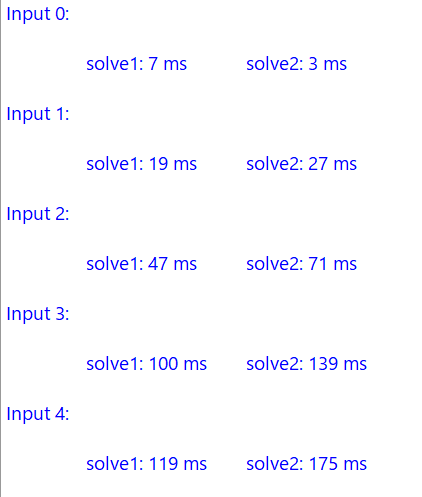
\includegraphics[width=7cm,height=7cm]{py1}
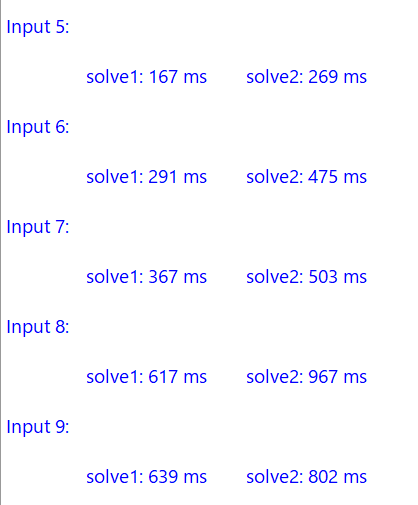
\includegraphics[width=7cm,height=7cm]{py2}
\end{figure}
\\Am observat c\u{a} solu\c{t}ia care folose\c{s}te o coad\u{a} are un timp mai mare de execu\c{t}ie fa\c{t}\u{a} de prima solu\c{t}ie. Acest lucru este datorat faptului c\u{a} implentarea cozii aloc\u{a} memoria diferit fa\c{t}\u{a} de rezolvarea \^{i}n care folosesc matrice.
\subsection{Concluzii}
\\ Aceast\u{a} tem\u{a} m-a ajutat s\u{a} \^{i}nteleg mai bine limbajul C \c{s}i \^{i}n special limbajul Python \^{i}n care mai lucrasem foarte pu\c{t}in p\^{a}n\u{a} acum  \c{s}i s\u{a} \^{i}mi aprofundez cuno\c{s}tin\c{t}ele pentru creearea de programe modulare.
\\ \^{I}n creearea temei am \^{i}nt\^{a}mpinat dificult\u{a}\c{t}i atunci c\^{a}nd am generat testele si le-am populat cu datele semnificative pentru problema mea, dar am reu\c{s}it sa scriu \c{s}i ulterior sa citesc datele din fiecare.
\\\^{I}n Python am reu\c{s}it s\u{a} salvez input-urile \c{s}i output-urile \^{i}ntr-un folder numit tests creat \^{i}n interiorul programului.
   
\section{Referin\c{t}e bibliografice}
\begin{itemize}
  \item [1.] {Data Structures and Algorithms in Python- autori: Michael T. Goodrich,Roberto Tamassia, Michael H. Goldwasser}
 
  \item [2.] $\href{https://www.geeksforgeeks.org/}{GeeksforGeeks}$
  \item [3.] $\href{https://docs.python.org//}{PythonDocs}$
  \item [4.] $\href{https://www.overleaf.com//}{Overleaf}$
  \item[4.]{Introduction to Algorithms-autori:  H. Cormen, Charles E. Leiserson, Ronald L. Rivest, Clifford Stein}
\end{itemize}
\end{document}